\section{CHAPTER 8: TRAPS AND CONTROL VALVES}
\subsection{Acquaintance}
Steam traps and control valves represent essential components in modern industrial operations, each serving distinct yet complementary functions in maintaining system efficiency. Steam traps operate as automatic filtering devices that remove unwanted condensate and non-condensable gases while preventing valuable steam from escaping the system. Control valves, functioning as flow regulators, adjust passage sizes based on signals received from system controllers, ensuring precise steam distribution throughout the network. Together, these components form a crucial partnership in industrial steam systems, effectively managing steam flow, preventing energy waste, and maintaining optimal operational conditions. Their combined operation significantly contributes to both system reliability and cost effectiveness, making them indispensable elements in contemporary industrial processes.

\subsection{Types of Steam Traps}
\subsubsection{Single Orifice Float Trap}

\textbf{Description:} Forbes Marshall's single orifice float trap enables condensate to drain out and retain steam. The body houses a simple yet effective mechanism, making the float trap perfect for fulfilling varied process needs. As the condensate gathers, the float rises to discharge it while ensuring that no steam is wasted in this process.
\begin{figure}[h]
    \centering
    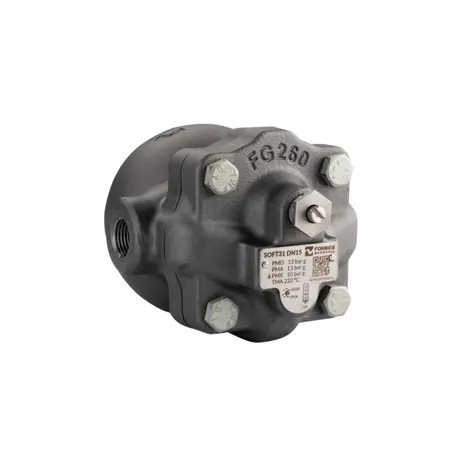
\includegraphics[width=0.8\textwidth,height=0.33\textheight,keepaspectratio]{figs/lastmin/Single Orifice Ball Float Trap.png}
    \caption{Single Orifice Float Trap}
    \label{fig:single_orifice_float_trap}
\end{figure}

\textbf{Features:}
\begin{enumerate}
    \item Effective and rapid condensate removal
    \item Traps steam in during normal operation, saving energy and reducing environmental effects
    \item Unique design allows flow to be directed away from critical parts to prevent wear and tear
    \item Anti-water hammer protection built into the design minimizes the risk of damage
\end{enumerate}

\subsubsection{Compact Module Two Orifice Float Trap}
\textbf{Description:}  This trap can deal with huge condensate amounts, especially at the time of startup when systems must warm up. Its dual orifice design makes it possible to accommodate small as well as large condensate loads without hesitation

\begin{figure}[h]
    \centering
    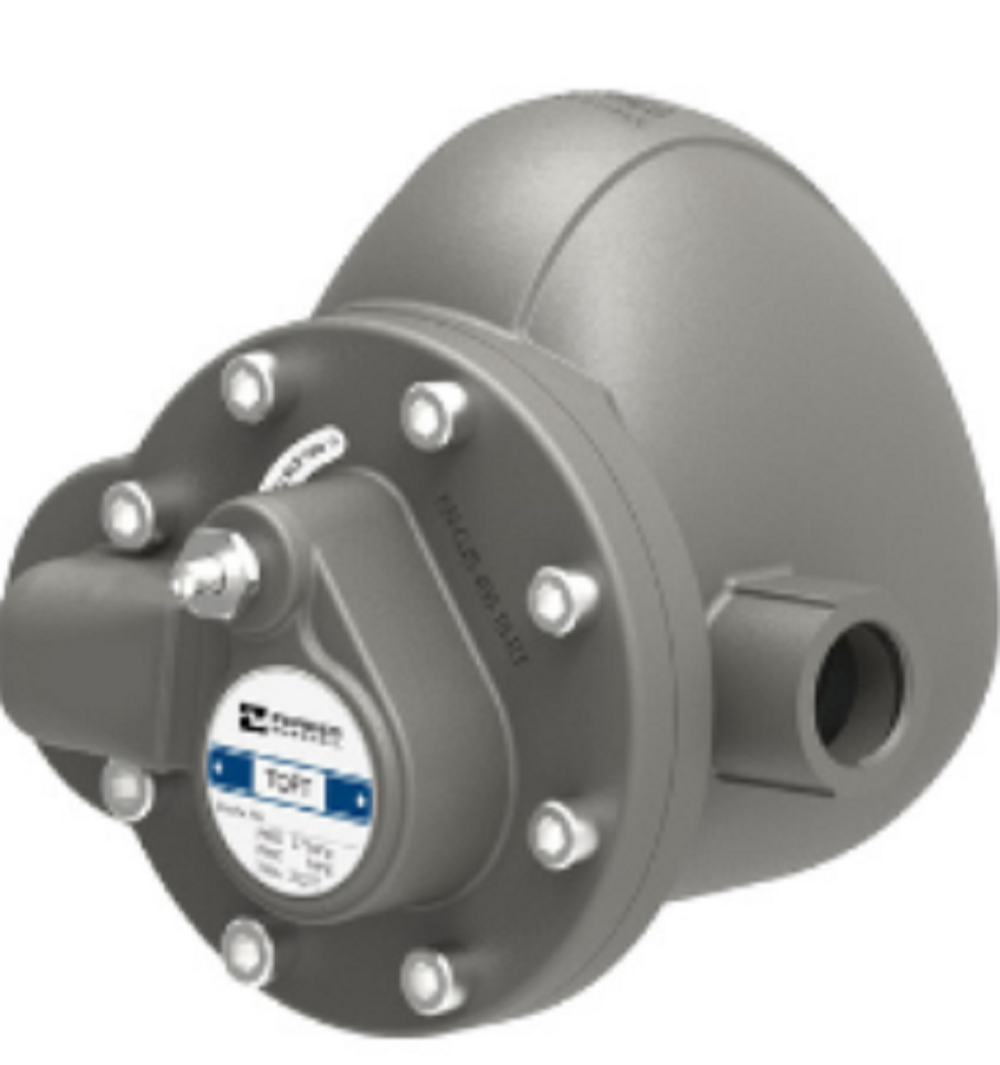
\includegraphics[width=0.8\textwidth,height=0.33\textheight,keepaspectratio]{figs/lastmin/two_orific_float_trap.png}
    \caption{Compact Module Two Orifice Float Trap}
    \label{fig:compact_module_two_orifice_float_trap}
\end{figure}

\textbf{Features:}
\begin{enumerate}
    \item Two openings, float-operated, one is for small loads, another one is used for large load
    \item All integral parts provide the elimination of trapped air and prevent the possibility of steam becoming trapped
    \item All-inclusive assembly in one compact package –strainer, check valve, and all the critical parts
    \item Special valves make sure nothing leaks out where it shouldn't
\end{enumerate}

\subsubsection{Thermodynamic Trap}
\textbf{Description:} These traps from Forbes Marshall stand up well to rust and corrosion while making sure condensate flows out smoothly. They’re built tough to last long in harsh conditions.

\begin{figure}[h]
    \centering
    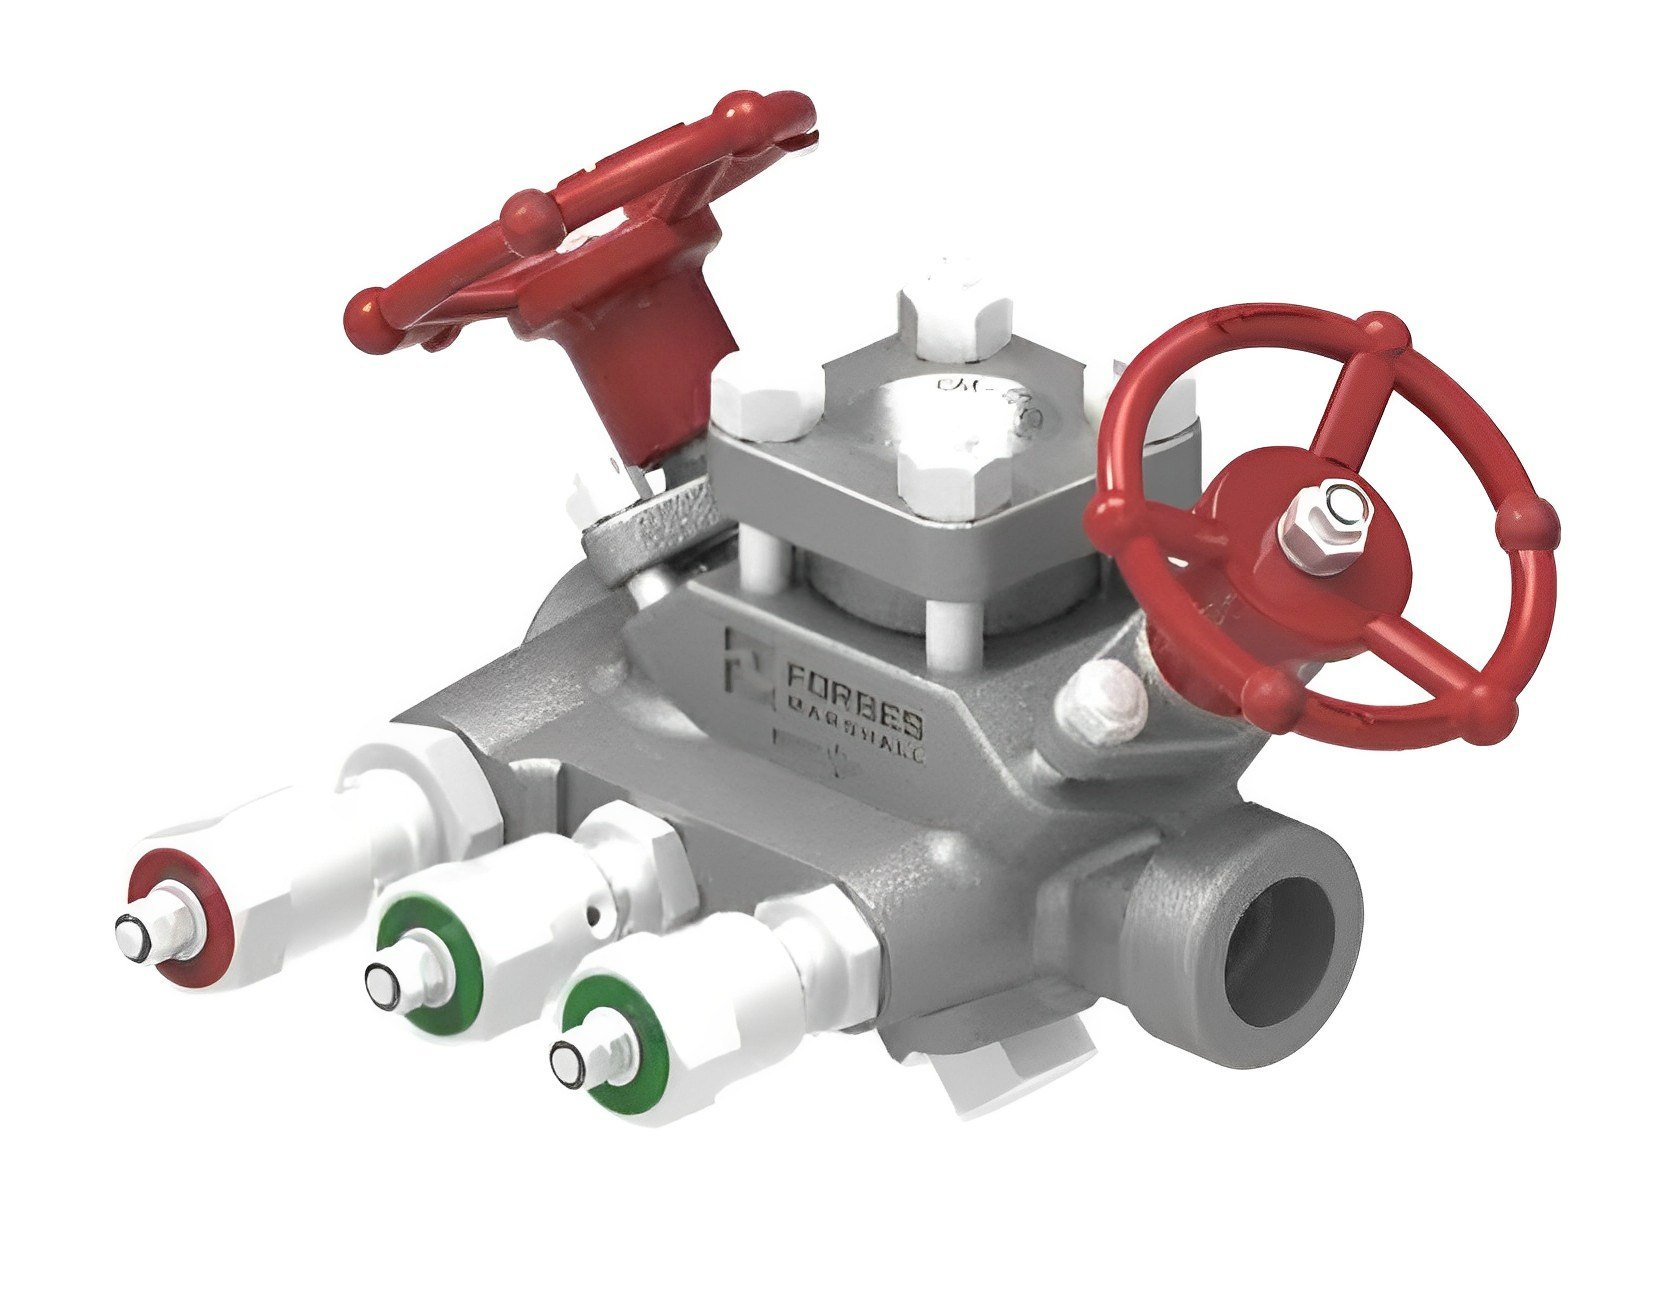
\includegraphics[width=0.8\textwidth,height=0.33\textheight,keepaspectratio]{figs/lastmin/thermodynamic_trap.png}
    \caption{Thermodynamic Trap}
    \label{fig:thermodynamic_trap}
\end{figure}

\textbf{Features:}
\begin{enumerate}
    \item Comes in different sizes and can connect to various pipe types
    \item Special discs are available to help prevent air from getting stuck inside
    \item Works well no matter what pressure you’re dealing with
    \item Extra-hard seating area means it lasts longer than regular traps
\end{enumerate}

\subsubsection{Compact Module Thermodynamic Trap}
\textbf{Description:} The heart of this module lies in how it brings together a thermodynamic steam trap and pipeline connector. It’s built smart, using a universal connector that makes everything work smoothly together.

\textbf{Features:}
\begin{enumerate}
    \item Everything lines up naturally in the pipe, making it simple to put in place
    \item Built tough with forged carbon steel that keeps going strong
    \item Gets up and running quickly - takes less than an hour to install
    \item Fits any way you need it to - no special angles needed
\end{enumerate}

\subsubsection{Bimetallic Trap}
\textbf{Description:} Forbes Marshall came up with this bimetallic steam trap to handle the tough stuff - it works great even when steam’s running hot and heavy through the lines.
\begin{figure}[h]
    \centering
    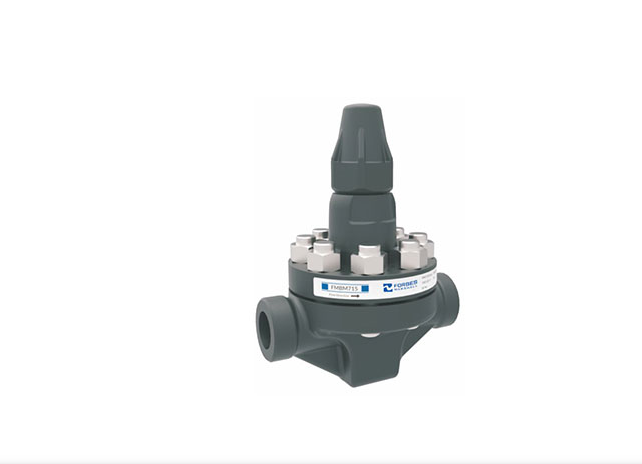
\includegraphics[width=0.8\textwidth,height=0.33\textheight,keepaspectratio]{figs/lastmin/bimetallic_thermostatic_steam_trap.png}
    \caption{Bimetallic Trap}
    \label{fig:bimetallic_trap}
\end{figure}


\textbf{Features:}
\begin{enumerate}
    \item Uses stainless steel parts inside to fight off wear and rust
    \item Keeps condensate in check with a smart valve system
    \item Catches all the junk with a built-in strainer
    \item Lets you fine-tune how hot things get with an adjustment screw
\end{enumerate}

\subsubsection{Bucket Traps}
\textbf{Description:} When you need to handle high-pressure condensate in horizontal pipes, these bucket traps from Forbes Marshall really shine. They’re built to handle the tough stuff while keeping things running smoothly.

\begin{figure}[h]
    \centering
    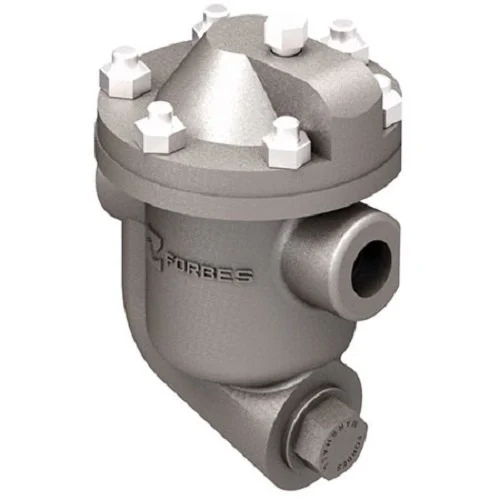
\includegraphics[width=0.8\textwidth,height=0.33\textheight,keepaspectratio]{figs/lastmin/bucket_trap.png}
    \caption{Bucket Trap}
    \label{fig:bucket_trap}
\end{figure}

\textbf{Features:}
\begin{enumerate}
    \item Stands up strong against water hammer
    \item Handles high pressure without breaking a sweat
    \item Keeps the system clean with its built-in strainer
\end{enumerate}

\subsection{Types of Control Valves}

\subsubsection{Globe Valves}
\textbf{Description:} Globe valves are a part of the flow control pipeline systems. Their robust construction makes it possible to achieve excellent shut-off characteristics, if not precisely controlled throttling in each kind of service application. 

\textbf{Features:}
\begin{enumerate}
    \item Excellent accuracy in controlling the flow
    \item Exhibits minimal leakage properties
    \item Proves good performance at high pressures
    \item Available with great material and dimensional diversity
\end{enumerate}

\subsubsection{Ball Valves}
\textbf{Description:} These valves provide good resistance to wear coupled with a high sealing performance. They are very effective when used in operations requiring fast operating times.

\begin{figure}[h]
    \centering
    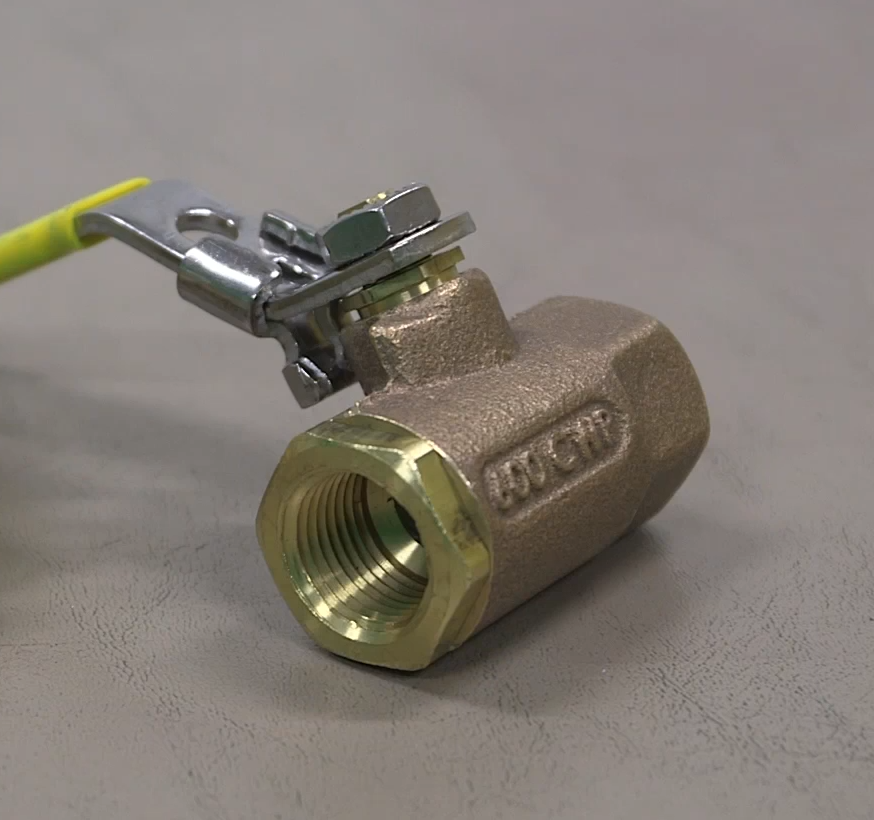
\includegraphics[width=0.8\textwidth,height=0.33\textheight,keepaspectratio]{figs/valves/ball.png}
    \caption{Ball Valve}
    \label{fig:ball_valve}
\end{figure}

\textbf{Features:}
\begin{enumerate}
    \item Permit fast operating - quarter-turn actuation
    \item Maintain optimum flow properties at minimum drop of pressure
    \item Sealing parts gives superior performance in a high range of temperatures and pressures.
    \item Available with a couple of arrangement types such as 2-way and 3-way etc.
\end{enumerate}

\subsubsection{Butterfly Valves}
\textbf{Description:} Butterfly valves are suitable to regulate and control the quantity of fluid.

\begin{figure}[h]
    \centering
    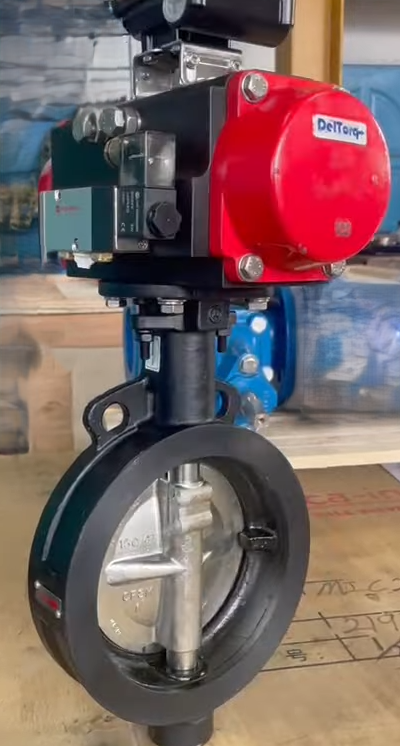
\includegraphics[width=0.8\textwidth,height=0.33\textheight,keepaspectratio]{figs/valves/butterfly.png}
    \caption{Butterfly Valve}
    \label{fig:butterfly_valve}
\end{figure}

\textbf{Features:}
\begin{enumerate}
    \item Permits efficient functioning with quarter-turn mechanism
    \item Provides inexpensive maintenance solutions
    \item Has proven particularly applicable for large-size applications
    \item Serves diverse fluid needs through material flexibility
\end{enumerate}

\subsubsection{Diaphragm Valves}
\textbf{Description:} Diaphragm valves are superb in performing, meeting specific applications requiring superior corrosion resistance. Its unique design makes it very advantageous when dealing with viscous fluids and slurry mixtures.

\textbf{Features:}
\begin{enumerate}
    \item Offers hermetic sealing properties
    \item Shows excellent resistance against abrasive and corrosive fluids
    \item Simplifies maintenance requirements
    \item Material configurations include custom elastomeric and poly-malic linings
\end{enumerate}

\subsubsection{Check Valves}
\textbf{Description:} These special flow control products ensure one-way fluid flow while preventing inverse flow conditions. Their application is important for equipment protection as well as the integrity maintenance of the system.

\textbf{Features:}
\begin{enumerate}
    \item Operates autonomously without external actuation requirements
    \item Presents low-pressure differential characteristics
    \item Utilizes disparate design versions, such as swing and lift mechanisms
    \item Can be installed either ina  horizontal or vertical position
\end{enumerate}

\subsubsection{Control Valves}
\textbf{Description:} The control valves are crucial equipment in process automation systems, which allow a very precise parameter adjustment of the flow, pressure, temperature variations and fluid level control in industrial processes.

\textbf{Features:}
\begin{enumerate}
    \item Allows for accurate modulation of process variables
    \item Allows easy integration into automated control systems
    \item Includes both linear and rotary actuation
    \item Proves to be flexible under different operating parameters and application demands
\end{enumerate}